\label{vier-gewinnt}

Vier Gewinnt ist ein Brettspiel, dessen Spielfeld aus 6 Zeilen und 7 Spalten besteht. Durch die beiden Spieler wird abwechselnd ein Spielstein in eine Spalte platziert, der in dieser Spalte bis zur untersten freien Position fällt. Es gewinnt der Spieler, durch den zuerst vier Spielsteine in einer horizontalen, vertikalen oder diagonalen Linie nebeneinander platziert wurden \cite{MiltonBradleyCompany.1990}. Abbildung \ref{fig:f23} zeigt eine diagonale Gewinnposition für den Spieler, der die blauen Steine platziert.

\begin{figure}
	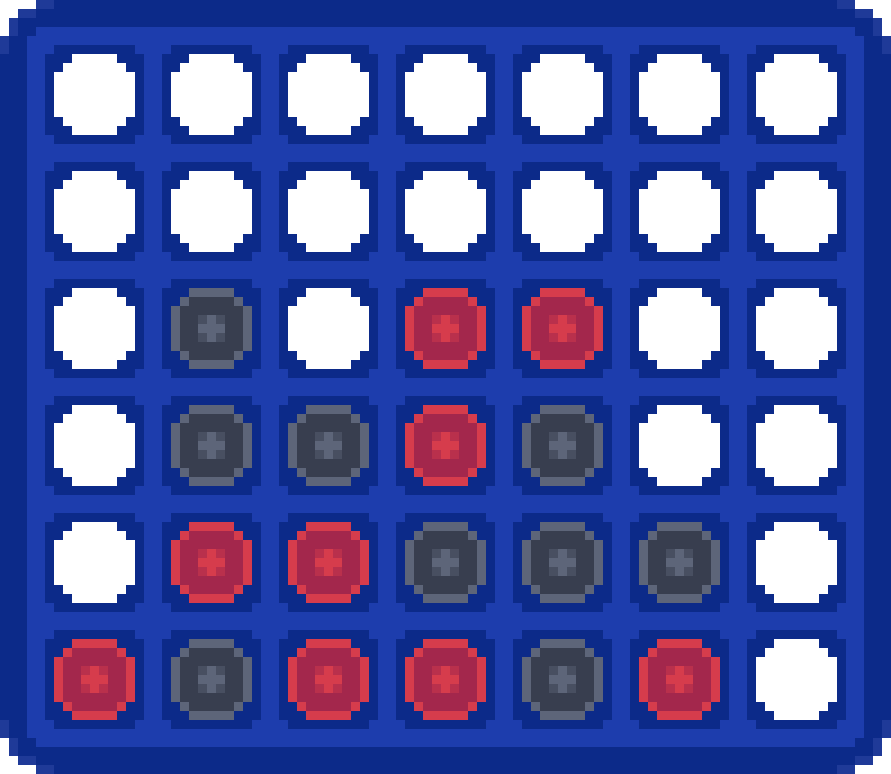
\includegraphics[width=0.5\textwidth, center]{Bilder/connect-four-boards/win-for-blue.png}
	\caption[Spielfeld von Vier Gewinnt mit einer diagonalen Gewinnposition für Blau.]{Spielfeld von Vier Gewinnt mit einer diagonalen Gewinnposition für Blau. Grafikdesign aus \cite{Farama.2025}.}
	\label{fig:f23}
\end{figure}

Bei Vier Gewinnt handelt es sich um ein kombinatorisches Nullsummenspiel für zwei Spieler. Kombinatorische Spiele weisen \glqq perfekte Information\grqq{} auf. Das bedeutet, dass alle Spieler zu jeder Zeit den gesamten Zustand des Spiels kennen. So ist es bei vielen Brettspielen der Fall. Kartenspiele hingegen besitzen diese Eigenschaft meistens nicht, weil jedem Spieler die Handkarten ihrer Gegenspieler unbekannt sind. Bei kombinatorischen Spielen sind außerdem keine Zufallselemente enthalten. Die einzige Herausforderung beim Spielen kombinatorischer Spiele besteht darin, unter einer Vielzahl von Entscheidungsoptionen diejenige auszuwählen, die für den Spieler den besten weiteren Spielverlauf verspricht (\cite{Bewersdorff.2018}, S. 96-100; \cite{Ferguson.January2019}, Kapitel 4.1).

Bei Zwei-Spieler-Nullsummenspielen verursacht der Sieg eines Spielers zwangsläufig die Niederlage des anderen Spielers. Die beiden Spieler haben damit entgegengesetzte Interessen (\cite{Bewersdorff.2018}, S. 100; \cite{Allis.1994}, S. 6). Das bedeutet, dass sich der Erfolg von verschiedenen Lösungsansätzen durch die durchschnittliche Gewinnrate im Spiel gegeneinander bewerten lässt. Bei Nullsummenspielen mit mehr als zwei Spielern, kann es passieren, dass eine (bewusst oder versehentlich) suboptimale Spielweise eines Spielers, dazu führt, dass ein zweiter Spieler davon profitiert, während ein dritter Spieler dadurch benachteiligt wird. Solche Wechselwirkungen sind bei Zwei-Personen-Nullsummenspielen ausgeschlossen (\cite{Bewersdorff.2018}, S. 113 ff.; \cite{Russell.2020}, S. 151 f.). Dadurch werden die Messergebnisse im Hauptteil besser vergleichbar.

\subsubsection{Markov Decision Process}

Vier Gewinnt lässt sich für beide Spieler jeweils als Markov Decision Process (MDP) modellieren. Dabei handelt es sich um ein Entscheidungsproblem, bei dem es darum geht, unter verschiedenen aufeinanderfolgenden und voneinander abhängigen Entscheidungsmöglichkeiten, die Beste zu wählen. Es hat folgende Bestandteile:

\begin{itemize}
	
\item Zustände $S$, die den legalen Spielfeldkonfigurationen entsprechen.
\item Aktionen $A(s)$, die für bestimmte Zustände erlaubt sind. In Vier Gewinnt existieren sieben verschiedene Aktionen, eine Aktion für jede Spalte, in der ein Spielstein platziert werden kann. Im Laufe des Spiels ändert sich, welche Aktionen möglich sind. In bereits vollständig gefüllten Spalten können keine weiteren Spielsteine platziert werden.
\item Übergangsmodell $P(s, a, s')$, das die Wahrscheinlichkeit beschreibt, von einem Zustand $s$ durch die Aktion $a$ zu einem weiteren Zustand $s'$ zu gelangen. Das Übergangsmodell hängt im Fall von kombinatorischen Spielen von der Strategie der anderen Spieler ab. Bei der Modellierung als MDP besteht die Annahme, dass sich die Strategie des Gegenspielers im Laufe des Spiels nicht ändert. Das Übergangsmodell ist dem Spieler nicht bekannt.
\item Belohnungsfunktion $R(s, a, s')$, wodurch jedem Zustandsübergang eine Belohnung zugeordnet wird. Bei einem Zwei-Spieler-Nullsummenspiel wie Vier Gewinnt beträgt dessen Wert 0, solange kein Endzustand erreicht ist. Wenn ein Endzustand erreicht ist, könnte diese Funktion beispielsweise einen positiven Wert zurückliefern, wenn der untersuchte Spieler gewinnt, und einen negativen Wert, wenn der Gegenspieler gewinnt.

\end{itemize}

Das Ziel bei der Lösung eines MDPs besteht darin, ein Regelwerk zu finden, das jedem Zustand jeweils eine Aktion zuordnet. Durch die Anwendung des Regelwerks soll die höchste erwartbaren Belohnung erzielt werden (\cite{Russell.2020}, S. 562 f.).

\subsubsection{Komplexität}

Nach Victor Allis lässt sich die Komplexität eines Spiels von strategiebasierten Zwei-Spieler-Nullsummenspielen durch ihre Zustandsraum- und Spielbaumkomplexität beschreiben. Die Zustandsraumkomplexität entspricht der Anzahl der verschiedenen möglichen Spielfeldkonfigurationen ab dem Start. Für Zwei-Spieler-Nullsummenspiele kann dieser Wert oder zumindest dessen obere Schranke bestimmt werden. Dazu werden zunächst alle Konfigurationen des Spielfelds gezählt, dann Einschränkungen wie Regeln und Symmetrie berücksichtigt, und die Anzahl der illegalen und redundanten Zustände von der Anzahl aller möglichen Konfigurationen abgezogen (\cite{Allis.1994}, S. 158 f.).

Die Spielbaumkomplexität beschreibt die Anzahl der Blattknoten des Lösungsbaums. Der Spielbaum ist ein Baum, der die Zustände eines Spiels als Knoten und die Züge als Kanten darstellt (\cite{Bewersdorff.2018}, S. 102; \cite{Russell.2020}, S. 147). Der Lösungsbaum beschreibt die Teilmenge des Spielbaums, der benötigt wird, um die Gewinnaussichten bei optimaler Spielweise beider Spieler zu berechnen. Die Spielbaumkomplexität lässt sich durch die durchschnittliche Spiellänge und der Anzahl der Entscheidungsmöglichkeiten pro Zug (entweder konstant oder abhängig vom Spielfortschritt) approximieren. Da in den meisten Spielen ein Zustand über mehrere Wege erreicht werden kann, fällt die Spielbaumkomplexität meist wesentlich größer aus als die Zustandsraumkomplexität (\cite{Allis.1994}, S. 159 ff.).

Die Spielbaumkomplexität ist maßgeblich für die praktische Berechenbarkeit einer starken Lösung. Für Tic Tac Toe wurde durch Allis eine obere Grenze für die Spielbaumkomplexität von 362880 ermittelt und eine starke Lösung lässt sich innerhalb von Sekundenbruchteilen berechnen \cite{Paul.2009}. Für Schach wird die Spielbaumkomplexität auf $10^{31}$ geschätzt und die Aussichten auf eine starke Lösung liegen noch in weiter Ferne \cite{Schaeffer.2007}.

Für Vier Gewinnt wurde eine durchschnittliche Spiellänge von 36 Zügen und eine durchschnittliche Anzahl von Entscheidungsmöglichkeiten (freie Spalten) von 4 ermittelt. Damit wurde die Spielbaumkomplexität auf $4^{36} \approx 10^{21}$ geschätzt (\cite{Allis.1994}, S. 163).

\subsubsection{Lösungsverfahren}

Für Vier Gewinnt wurden bereits verschiedene Lösungsverfahren ausgiebig untersucht. Das Spiel wurde 1988 von James Dow Allen und Victor Allis unabhängig voneinander mit wissensbasierten Methoden schwach gelöst, was bedeutet, dass für die Anfangsposition eine optimale Strategie ermittelt wurde. Im Fall von Vier Gewinnt kann der Spieler mit Anzugsrecht bei optimaler Spielweise immer gewinnen \cite{Allen.2010} \cite{Allis.1988}. Der Begriff Anzugsrecht bezeichnet das Recht eines Spielers, den ersten Zug durchführen zu dürfen, und in dieser Arbeit in Anlehnung an (\cite{Bewersdorff.2018}) verwendet.

1993 wurde das Spiel von John Tromp auch durch einen Brute-Force Ansatz stark gelöst. Bei dieser Lösung kam Alpha-Beta-Pruning zum Einsatz, um bei einer Zustandsraumkomplexität von 4.531.985.219.092 die optimalen Zugfolgen für beide Spieler zu berechnen. Das hat damals etwa 40.000 CPU-Stunden gedauert \cite{Tromp}.

Lösungen, die alle Möglichkeiten durchrechnen, um die optimale Entscheidung zu treffen, sind für den Einsatz in der Praxis aufgrund des hohen Rechenaufwands bei komplexeren Anwendungen auch heute noch selten praktikabel. Aus diesem Grund wird bevorzugt auf gute Heuristiken zurückgegriffen, die den Rechenaufwand minimieren, aber dennoch gute Ergebnisse liefern (\cite{Heineman.October2008}, Kapitel 7.6).

Untersuchungen haben gezeigt, dass sich sowohl regelbasierte Algorithmen als auch verschiedene RL-Ansätze eignen, um sogenannte Agents zu entwickeln, die das Spiel selbstständig spielen \cite{Thill.2012} \cite{Wäldchen.2022} \cite{Taylor.2024} \cite{Sheoran.2022} \cite{Qiu.2022}. Wissensbasierte Methoden werden in dieser Arbeit nicht näher betrachtet, da sie stark an die jeweiligen Spielregeln gebunden und ihre Eigenschaften schwer zu verallgemeinern sind.
